\begin{center}
	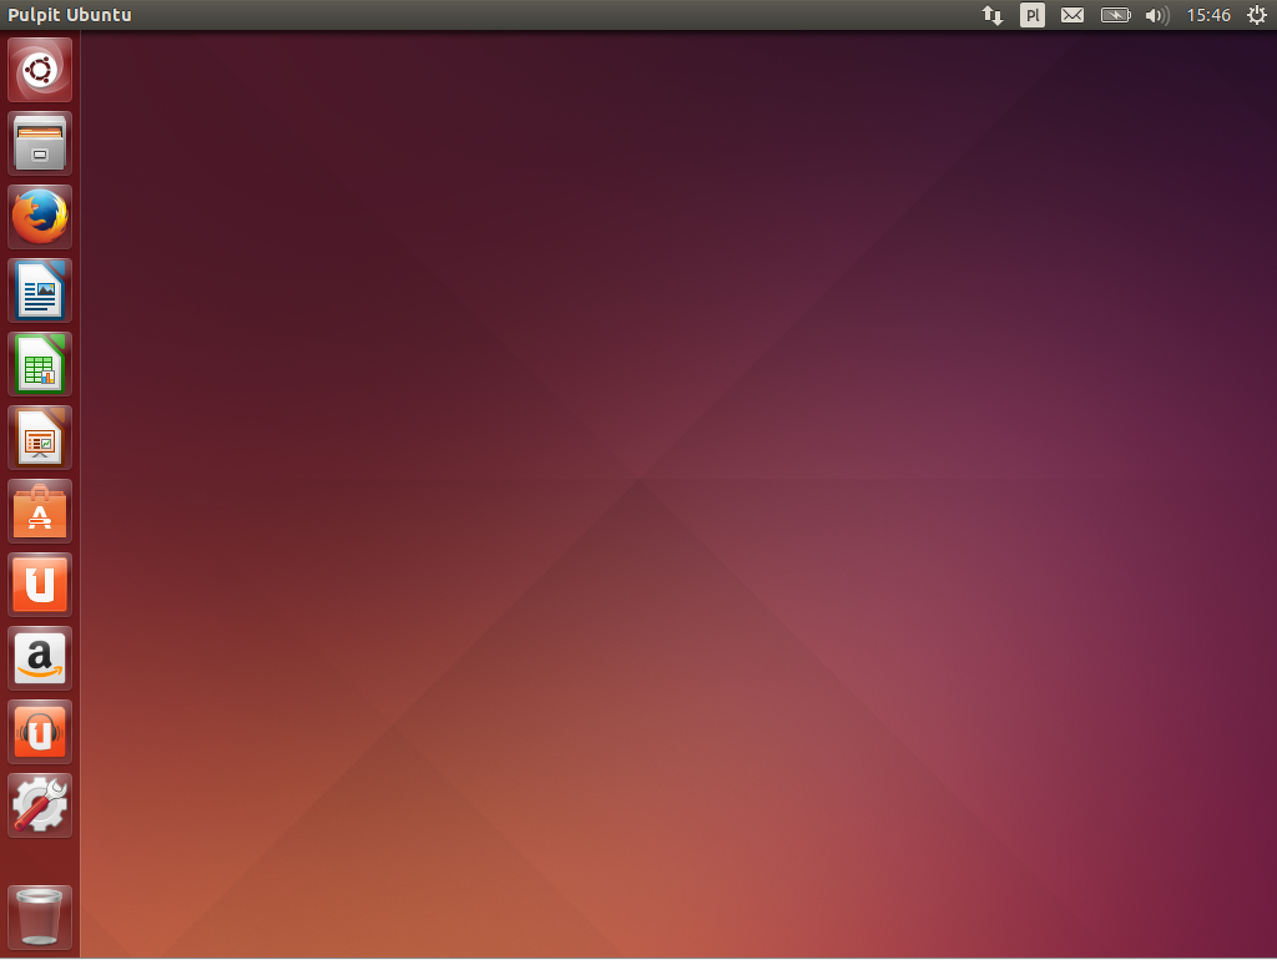
\includegraphics[scale=0.4]{images/unity_desktop.png}
\end{center}

Po zalogowaniu się do systemu Twoim oczom ukaże się Pulpit. Widać na nim trzy elementy: przestrzeń roboczą wypełniającą większą część ekranu oraz dwa panele. Panel poziomy, zwany \textbf{panelem menu}, umieszczony na górze ekranu. Panel pionowy to \textbf{Launcher}, zlokalizowany jest po lewej stronie ekranu.
\clearpage

\subsubsection{Zmiana tła pulpitu}
Aby zmienić tło pulpitu (inaczej: tapetę) kliknij \textbf{prawym przyciskiem myszy} na wolnej przestrzeni roboczej i z menu kontekstowego wybierz "Zmień tło pulpitu"

\begin{wrapfigure}{r}{0.5\textwidth}
                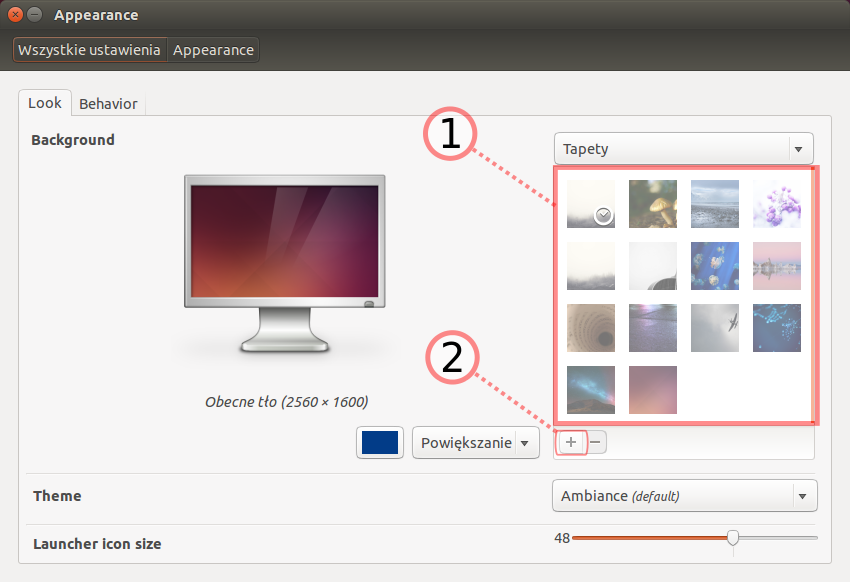
\includegraphics[width=\linewidth]{images/unity_zmiana_tapety.png}
\end{wrapfigure}

Z listy zaznaczonej jako (1) możesz wybrać jedną z gotowych tapet. Kliknij na przycisk + (2) aby otworzyć menadźer plików i wskazać inny plik graficzny na dysku twardym. Plik ten zostanie użyty jako tapeta.

W tym oknie możesz też dokonać pewnych modyfikacji środowiska graficznego Unity. Zachęcamy do eksperymentów. Wszelkie zmiany są wprowadzane na żywo.
\clearpage

